\section{tasks::plotspec Class Reference}
\label{classtasks_1_1plotspec}\index{tasks::plotspec@{tasks::plotspec}}
Inheritance diagram for tasks::plotspec::\begin{figure}[H]
\begin{center}
\leavevmode
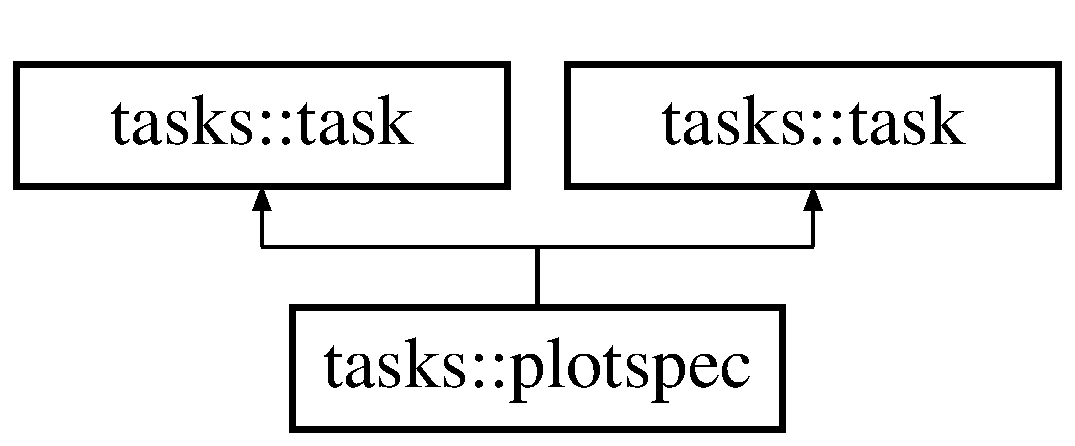
\includegraphics[height=2cm]{classtasks_1_1plotspec}
\end{center}
\end{figure}
\subsection*{Public Member Functions}
\begin{CompactItemize}
\item 
def \textbf{run}\label{classtasks_1_1plotspec_2ec7ebb6665b3d10b3a687b9666a323b}

\item 
def \textbf{run}\label{classtasks_1_1plotspec_2ec7ebb6665b3d10b3a687b9666a323b}

\end{CompactItemize}
\subsection*{Static Public Attributes}
\begin{CompactItemize}
\item 
string \textbf{name} = '{\bfplotspec}'\label{classtasks_1_1plotspec_7c593740af4fa1d7488bab919fe923c9}

\item 
string \textbf{button\-Text} = 'Plot reduced spectrum'\label{classtasks_1_1plotspec_046297279c378a693ed8e6122d8b84cb}

\item 
int \textbf{inthread} = 0\label{classtasks_1_1plotspec_cffba8dccd1d76c830747d71462c4681}

\end{CompactItemize}


\subsection{Detailed Description}


\footnotesize\begin{verbatim}Plot (part of) an extracted spectrum.
\end{verbatim}
\normalsize
 



The documentation for this class was generated from the following files:\begin{CompactItemize}
\item 
old/PANICtool-1.0/tasks.py\item 
old/tasks.py\end{CompactItemize}
